% Fruit Ninja VR - Part 2 - Rapport (mise en page sobre, texte simplifie)
% Compilation : pdflatex x2
\documentclass[11pt,a4paper]{article}

\usepackage[T1]{fontenc}
\usepackage[utf8]{inputenc}
\usepackage{lmodern}
\usepackage[french]{babel}
\usepackage[a4paper,margin=2.2cm]{geometry}
\usepackage{graphicx}
\usepackage{booktabs}
\usepackage{tabularx}
\usepackage{array}
\usepackage{enumitem}
\usepackage{caption}
\usepackage{float}
\usepackage{fancyhdr}
\usepackage[hidelinks]{hyperref}

\setlist{nosep,leftmargin=*}
\captionsetup{font=small,labelfont=bf}
\setlength{\parskip}{0.4em}
\setlength{\parindent}{0pt}
\renewcommand{\arraystretch}{1.15}
\newcolumntype{L}{>{\raggedright\arraybackslash}X}
\newcolumntype{P}[1]{>{\raggedright\arraybackslash}p{#1}}
\newcommand{\fichier}[1]{\texttt{\small #1}}
\emergencystretch=2em
% Autorise les césures après / et - dans les chemins \texttt (sinon débordements).
\makeatletter
\renewcommand{\texttt}[1]{%
  {\ttfamily\hyphenchar\font=`\/ \hyphenpenalty=50 \exhyphenpenalty=50 #1}}
\makeatother

\pagestyle{fancy}
\fancyhf{}
\lhead{\small Fruit Ninja VR : Part 2}
\rhead{\small Junghoon KIM, ST2VAAS 2026-2027}
\cfoot{\small \thepage}

\begin{document}

\begin{center}
  {\LARGE\bfseries Fruit Ninja VR : Part 2}\\[4pt]
  {\Large Gestion des ressources et optimisation mémoire}\\[10pt]
  ST2VAAS 2026-2027, Junghoon KIM\\[4pt]
  Dépôt : \url{https://github.com/Ethervel/FruitNinjaVR}, branche \texttt{part2}\\[2pt]
  {\small Unity 6000.0.56f1, URP 17.0.4, Addressables 2.10.3, OpenXR 1.15.1}
\end{center}

\textbf{Résumé.} La Part 2 remplace les créations et destructions d'objets pendant le jeu
par des réserves d'objets réutilisés (pools). Elle charge aussi les effets et le sabre
selon la plateforme (PC VR ou Quest). Les mesures PC et Quest montrent moins d'allocations
mémoire et plus aucun objet détruit en jeu.

Les mesures Quest viennent de la session casque du 25/11 (Quest 3 porté, écran à
72~Hz). Le scénario de test n'est pas le même sur Quest et sur PC : le bench Quest
coupe 13 à 37 fruits par partie au lieu de 34, donc les chiffres Quest sont aussi
donnés par coupe et par minute (section~\ref{sec:mesures}). Les figures sont des
graphiques tracés à partir des mesures du jeu, pas des captures d'écran du Profiler
(l'outil de mesure de Unity) : l'éditeur n'était pas ouvert pendant les runs Quest,
et \texttt{adb screencap} est bloqué sur Quest 3. Les tests visuels Quest et PCVR
via Link sont confirmés par l'utilisateur (déclaratif) ; les journaux ne couvrent
qu'une partie du test Quest et ne montrent pas le test PCVR
(section~\ref{sec:tests}).

% =====================================================================
\section{Objectif et méthode}

Dans la Part 1, le jeu fonctionnait sur PC VR et Quest. Mais chaque fruit, bombe, effet
et morceau de fruit était créé puis détruit pendant la partie. Sur le scénario de test,
cela faisait environ 424 créations/destructions (\texttt{Instantiate}/\texttt{Destroy}),
242,6~Mo d'allocations mémoire et 145 ramasse-miettes.

Le GC (« garbage collector », ramasse-miettes) est le mécanisme qui libère la mémoire
des objets C\# oubliés. Chaque collecte prend du temps processeur et peut provoquer une
micro-saccade. Réduire les allocations réduit les collectes.

Le travail suit les tâches du sujet. Task 1 : pools des objets de jeu (fruits,
bonus, bombes). Task 2 : pools des effets et des morceaux, avec réutilisation des
meshes. Tasks 3 et 4 : Addressables, le système de Unity qui charge des assets
(prefabs, textures...) depuis des fichiers séparés (bundles), choisis au build.
Ici il sert à charger la variante PCVR ou Quest des effets et du sabre.

Pour comparer l'avant et l'après, un mode de test automatique (le bench,
\fichier{Assets/Scripts/Debug/}\allowbreak\fichier{BenchMode.cs}) rejoue toujours la même partie :
graine aléatoire fixe 12345, difficulté Normal, une coupe simulée toutes les 0,35~s,
une bombe touchée jusqu'à explosion après 15~s, 3 parties séparées par 2 retours au menu.
La coupe simulée passe par le même code que le sabre du joueur.

Le bench s'active par \texttt{-bench} sur PC et par extra d'intent (\texttt{am start
\ldots{} -e bench 1}) sur Quest. Il mesure chaque frame avec \texttt{ProfilerRecorder},
une API de Unity qui lit les compteurs du Profiler depuis le jeu (temps CPU, mémoire
allouée, mémoire utilisée). Il écrit trois fichiers : \texttt{bench-summary.json},
\texttt{frames.csv} (une ligne par frame) et \texttt{summary.csv}.

Les deux builds de référence sont archivés dans \fichier{Builds/Bench/avant|apres/} :
« avant » = Part~1 + bench, « après » = état final. Les deux sont en mode Development
avec connexion Profiler activée.

% =====================================================================
\section{Task 1 : pools de fruits et bombes}

\subsection{Organisation}

Un pool est une réserve d'instances désactivées. Au lieu de créer un fruit, le jeu en
active un du pool ; au lieu de le détruire, il le range. Il y a un pool par prefab
(\fichier{GameObjectPool.cs}, \fichier{PoolManager.cs}) : 8 fruits ordinaires, le fruit
bonus et la bombe. Une instance ne change jamais de type.

Les stocks de départ viennent des pics mesurés sur l'état « avant » :

\begin{table}[H]
\centering\small
\caption{Stocks initiaux et pics observés au bench (3 parties).}
\begin{tabularx}{\textwidth}{@{}P{3.4cm}P{2cm}P{2.6cm}L@{}}
\toprule
Pool & Stock & Pic d'usage & Justification \\
\midrule
Chaque fruit ordinaire ($\times 8$) & 4 & 1 à 2 & pic global 3 fruits vivants, réparti sur 8 variétés ; 4 couvre les rafales \\
Fruit bonus & 2 & 1 & 7~\% des spawns \\
Bombe & 4 & 2 & $\approx 10$~\% des spawns, durée de vie longue (10~s + explosion) \\
\bottomrule
\end{tabularx}
\end{table}

Au bench « après » : 42 créations (= les stocks, aucune croissance), 111 réutilisations
pour les fruits/bonus/bombes, aucun \texttt{Destroy} en jeu. Les pools peuvent grandir
si une difficulté plus rapide l'exige (\texttt{maxSize} = 0 par défaut).

\subsection{Remise à zéro à la réactivation}

L'objet est remis à neuf quand il sort du pool (\texttt{Get}), pas quand il rentre.
L'objet rangé garde son dernier état, ce qui aide au debug. Rien de l'usage précédent
ne passe au suivant :

\begin{itemize}
\item Transform : position et rotation demandées, échelle du prefab restaurée.
\item Physique : vitesses à zéro, \texttt{isKinematic} et contraintes remis à neuf,
      \texttt{Sleep()}. La coroutine de gravité du spawner est neutralisée au retour
      (compteur de génération + \texttt{InUse}).
\item Colliders : état restauré depuis le prefab (un morceau n'a qu'un collider actif
      sur trois) ; réactivés pour les fruits et bombes.
\item Apparence : renderers réactivés, particules stoppées et vidées.
\item Données de jeu (via \texttt{OnEnable}) : \texttt{wasSliced} remis à faux ;
      bombe : compteur de touches, état d'explosion, flash (alpha 0, quad caché).
      Le timeout de 10~s (\fichier{PooledLifetime.cs}) est réarmé à chaque activation
      et annulé à la désactivation.
\end{itemize}

\subsection{Retours au pool et gardes}

Tous les \texttt{Destroy} du gameplay sont devenus des retours au pool : coupe
(\texttt{Slicer}), sol (\texttt{DestroyFloor}), chute sous $y=-2$, nettoyage de fin de
partie (\texttt{FruitSpawner}, \texttt{GameManager}), timeout 10~s, et bombe après
explosion. Avant, la bombe explosée restait figée dans la scène. La vraie destruction
n'a lieu qu'à l'arrêt ou au déchargement de la scène (\texttt{DestroyAll} ; le quad et
le matériau du flash de la bombe sont détruits explicitement).

Deux gardes protègent le score :
\begin{itemize}
\item \texttt{FruitController.TryMarkSliced} est partagée par les deux sabres. Un fruit
      touché par les deux ne compte qu'une fois. Avant, le \texttt{HashSet} local de
      chaque sabre ne couvrait que lui-même, et une seule frame.
\item \texttt{BombController.StartExplosionSequence} refuse une seconde séquence :
      une bombe = une pénalité d'explosion.
\end{itemize}

Le bench vérifie 3 parties sans état résiduel : 34 coupes, 3 touches et 1 explosion
par partie, identiques d'une partie à l'autre.

% =====================================================================
\section{Task 2 : pools d'effets et de morceaux}

Les effets (\fichier{GameFX.cs}) ont un pool par variante (jus : 8, explosions : 4).
Ces stocks couvrent les pics mesurés : 5 jus simultanés au bench, 3 effets par bombe.
À la sortie du pool : \texttt{Stop(StopEmittingAndClear)} + \texttt{Clear(true)} puis
\texttt{Play(true)}. Aucune particule de l'usage précédent ne subsiste. Le retour au
pool est programmé à la fin de l'effet (\texttt{FXReturn}, durée + 0,5~s) ; il remplace
\texttt{Destroy(fx, délai)}. Au bench : 8 + 4 créations, 102 + 6 réutilisations.

Les morceaux de fruits (\fichier{Slicer.cs}, \fichier{SlicedPiece.cs}) viennent d'un
pool de 24 objets créés depuis un template (pic mesuré : 6 au bench, $\approx 15$
estimés en jeu réel). Chaque morceau garde son Mesh (le maillage 3D). Il est réécrit à chaque
coupe (\texttt{Clear()} puis \texttt{SetVertices/SetNormals/SetUVs/SetTriangles}) au
lieu d'un \texttt{new Mesh}. L'allocation GPU est donc réutilisée. La géométrie de
découpe (plan, caps, triangulation) est inchangée.

Les composants physique sont réutilisés : Rigidbody et un collider primitif actif,
reconfiguré selon la forme. Plus d'\texttt{AddComponent} par coupe. Les matériaux de
cap (la face colorée du morceau) sont mis en cache par couleur : la palette des fruits
est fixe. Au bench : 24 créations, 204 réutilisations, 204 retours. Avant : 204
créations et 204 destructions.

% =====================================================================
\section{Tasks 3 et 4 : Addressables et variantes du sabre}

\subsection{Groupes et cycle de vie}

Paquet \texttt{com.unity.addressables} 2.10.3. Deux groupes : \texttt{FX\_PCVR}
(Windows) et \texttt{FX\_Quest} (Android). Les adresses sont les mêmes dans les deux
groupes : \texttt{FX\_FruitJuice}, \texttt{FX\_BombExplosion}, \texttt{Katana}. Le code
charge donc les mêmes clés partout. C'est le catalogue du build qui pointe vers le
bundle de sa plateforme.

Chaque groupe n'est inclus que dans le build de sa plateforme (\texttt{IncludeInBuild},
piloté par \texttt{AddressablesSetup.SetPlatform}). Les chemins sont distincts :
\texttt{aa/PCVR/} et \texttt{aa/Quest/}.

Cycle de vie (\fichier{AssetLoader.cs}) :
\begin{itemize}
\item \texttt{LoadAssetAsync} avant la première partie (le bench attend \texttt{IsReady}).
\item Les pools d'effets sont alimentés avec les assets chargés.
\item Le handle (la référence qui maintient l'asset en mémoire) est gardé tant que des
      clones existent : ils utilisent les meshes et matériaux du bundle.
\item À l'arrêt, les instances sont détruites, puis les handles libérés. La libération
      est différée d'une frame pour garantir cet ordre.
\item En cas d'échec : journalisation, libération du handle raté, repli sur des
      références directes. Le jeu reste jouable.
\end{itemize}

Le contenu est généré pour Windows et Android.

Test d'échec (simulé sur PC, \texttt{-benchFailAssets}) : les trois chargements échouent
(\texttt{InvalidKeyException}), le repli prend le relais, le bench complète ses 3
parties avec le même score. Détail et logs : \fichier{docs/part2/addressables.md} et
\fichier{docs/part2/mesures-apres/echec-assets/}.

\subsection{Katana : deux variantes}

\begin{table}[H]
\centering\small
\caption{Variantes du katana, chargées par Addressables selon la plateforme.}
\begin{tabularx}{\textwidth}{@{}P{2.2cm}P{3.4cm}P{3.2cm}L@{}}
\toprule
 & PCVR & Quest & \\
\midrule
Mesh & 1275 sommets / 851 triangles (FBX d'origine) & 132 sommets / 260 triangles ($\approx 31$~\%), asset 14~ko & decimation editor (clustering 1,5~\%, triangles dégénérés supprimés, normales recalculées) \\
Matériaux & matériaux d'origine du modèle (7 slots) & 1 matériau URP Simple Lit sans texture & une passe de shading, pas de maps \\
Application & visuel identique à la Part 1 & \texttt{KatanaVariant\allowbreak Applier} remplace mesh, matériaux et collider des sabres & le GameObject du sabre (rig XR) n'est pas remplacé \\
\bottomrule
\end{tabularx}
\end{table}

\subsection{Contenu du build et contenu chargé en mémoire}

Le contenu du build est ce qui est livré : les bundles de la plateforme active, le
catalogue, et les assets référencés directement par les scènes (fruits, bombes, décor,
replis). L'autre variante n'est pas dans le build.

Le contenu chargé en mémoire est ce qui réside à l'exécution. Un bundle sur le disque
ne coûte rien tant qu'il n'est pas chargé. \texttt{LoadAssetAsync} le charge ; le handle
le maintient en mémoire. Les clones des pools ne dupliquent pas les meshes : ils les
référencent. \texttt{Release} décharge quand plus aucun clone n'en dépend. La taille du
build dépend des groupes inclus. La mémoire dépend des handles actifs et des stocks
préchauffés.

% =====================================================================
\section{Protocole et mesures}\label{sec:mesures}

Machine PC : i9-14900KF, RTX 3080, 32~Go, Windows 11. Unity 6000.0.56f1. Builds
Development + Deep Profiling, lancés en \texttt{-batchmode -nographics} (sans fenêtre
ni casque). Les mesures viennent de \texttt{ProfilerRecorder} dans le build : une ligne
par frame dans \texttt{frames.csv}. Protocoles détaillés :
\fichier{docs/part2/mesures-avant/protocole.md} et
\fichier{docs/part2/mesures-apres/protocole.md}.

\begin{table}[H]
\centering\small
\caption{Comparatif PC avant/après (3 parties, même seed, même séquence).}
\begin{tabularx}{\textwidth}{@{}L P{2.6cm} P{2.6cm}@{}}
\toprule
Indicateur & Avant & Après \\
\midrule
CPU moyen (ms) & 0,39 & 0,37 \\
CPU p95 / p99 (ms) & 0,55 / 0,70 & 0,44 / 0,56 \\
CPU max (ms, pic de chargement) & 42,3 & 43,9 \\
Allocations GC totales (Mo) & 242,6 & 224,9 \\
Alloc moyenne (ko/frame) & 1,02 & 0,90 \\
Collectes GC gen0 & 145 & 134 \\
Mémoire utilisée fin de bench (Mo) & 110,9 & 103,8 \\
\texttt{Instantiate} réels sur le scénario & 424 & 74 (= stocks) \\
Réutilisations de pools & 0 & 423 \\
\texttt{Destroy} en jeu & 424 & 0 \\
Fruits coupés / partie (contrôle) & 34 & 34 \\
Score / partie (contrôle, $\times 3$) & 895 & 815 (voir ci-dessous) \\
\bottomrule
\end{tabularx}
\end{table}

\begin{itemize}
\item Score 895 $\rightarrow$ 815 : les bombes explosées ne restent plus figées dans
      la scène. Le bench re-touche alors une nouvelle bombe, d'où des pénalités en plus.
      C'est le comportement correct face à un joueur réel : l'« avant » profitait d'un
      état résiduel. Les fruits coupés et la séquence de spawn sont identiques.
\item CPU max 43,9~ms et pic d'allocation 243,3~ko/frame : c'est le chargement
      Addressables au démarrage (une seule fois, phase \texttt{loading}). Ce n'est pas
      une régression en jeu, et les p95/p99 baissent.
\item CPU moyen quasi stable (0,39 $\rightarrow$ 0,37~ms) : sans casque, le bench est
      dominé par le rendu et la simulation, pas par les allocations. Le gain se voit
      surtout sur la mémoire et les collectes, et au casque (IL2CPP, mémoire plus
      contrainte).
\end{itemize}

\subsection{Mesures Quest (casque porté, 72 Hz)}

Quest 3, Android 14 (vOS 205), APK Development + connexion Profiler, bench seed 12345,
3 parties + 2 retours menu.

Le scénario n'est pas identique entre runs. À 72~fps, les fruits montent moins haut
entre deux frames. Ils passent moins de temps au-dessus du seuil de coupe du bench, et
les 3 vies se perdent plus tôt. Le run avant fait 51 coupes en 70,7~s ; le run après,
75 coupes en 77,4~s. Les chiffres bruts ne se comparent donc pas tels quels. Pour comparer, je regarde
les lignes normalisées du tableau : par coupe et par minute.

Une frame a duré 10,7~s pendant le run avant (événement du système Quest, absent des
deux autres runs). Elle est exclue des moyennes.

\begin{table}[H]
\centering\small
\caption{Comparatif Quest avant/après (runs de référence ; $\dagger$ = normalisé).}
\begin{tabularx}{\textwidth}{@{}L P{2.6cm} P{2.6cm}@{}}
\toprule
Indicateur & Avant (Quest) & Après (Quest) \\
\midrule
Frames / durée (s) & 4275 / 70,7 & 5541 / 77,4 \\
Coupes totales (3 parties) & 51 & 75 \\
CPU moyen / p95 (ms) & 13,95 / 14,57 & 13,91 / 14,38 \\
CPU p99 / max hors pic (ms) & 15,06 / 213 & 14,83 / 303 \\
Alloc GC moyenne (ko/frame) & 1,37 & 1,17 \\
Alloc GC par coupe$^\dagger$ (ko) & 115,0 & 86,8 ($-25$~\%) \\
Alloc GC par minute$^\dagger$ (Mo) & 4,86 & 4,93 \\
Collectes GC (total / par minute$^\dagger$) & 28 / 23,8 & 38 / 29,4 \\
\texttt{Instantiate} réels & à la demande (57 fruits) & 74 (= stocks) \\
Réutilisations de pools & 0 & 322 \\
\texttt{Destroy} en jeu & oui (57 fruits, 102 morceaux) & 0 \\
Mémoire utilisée fin (Mo, CSV) & 845,0 & 893,8 ($+50$ = stocks) \\
VrApi FPS / App / CPU\&GPU (ms) & 72/72 ; 8,62 ; 13,31 & 72/72 ; 8,87 ; 12,44 \\
\bottomrule
\end{tabularx}
\end{table}

\begin{itemize}
\item Les allocations GC par coupe baissent de 25~\%.
\item 74 créations au démarrage (= les stocks), 322 réutilisations, 0 destruction en jeu.
\item Le CPU moyen est stable ($\sim$13,9~ms) : il est dominé par le rendu à 72~Hz.
      Le temps CPU\&GPU mesuré par VrApi (l'API système du Quest) baisse un peu :
      13,31 $\rightarrow$ 12,44~ms.
\item La mémoire gagne $\sim$50~Mo : c'est la pré-allocation des stocks au démarrage,
      pas une fuite. Ensuite la croissance est quasi nulle (+0,5~Mo sur les 2000
      dernières frames). Tous les pics d'usage restent sous les stocks.
\item Les collectes par minute montent un peu (29,4 contre 23,8) car le run après est
      plus actif (75 coupes contre 51). Le coût par coupe, lui, baisse.
\end{itemize}

\begin{figure}[H]
\centering
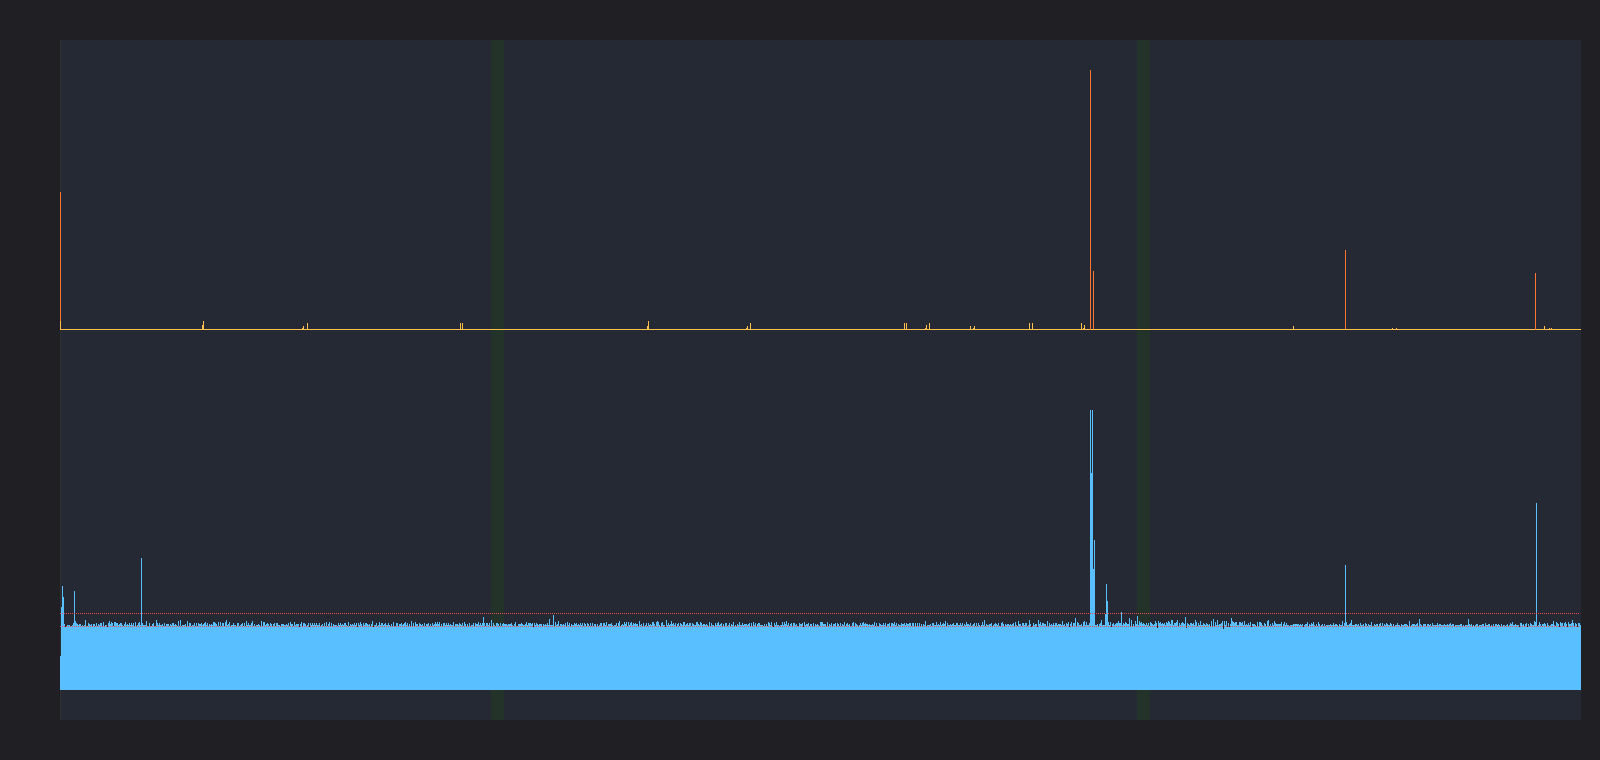
\includegraphics[width=\textwidth]{../captures-profiler/quest-avant-profiler-synthese.png}\\[4pt]
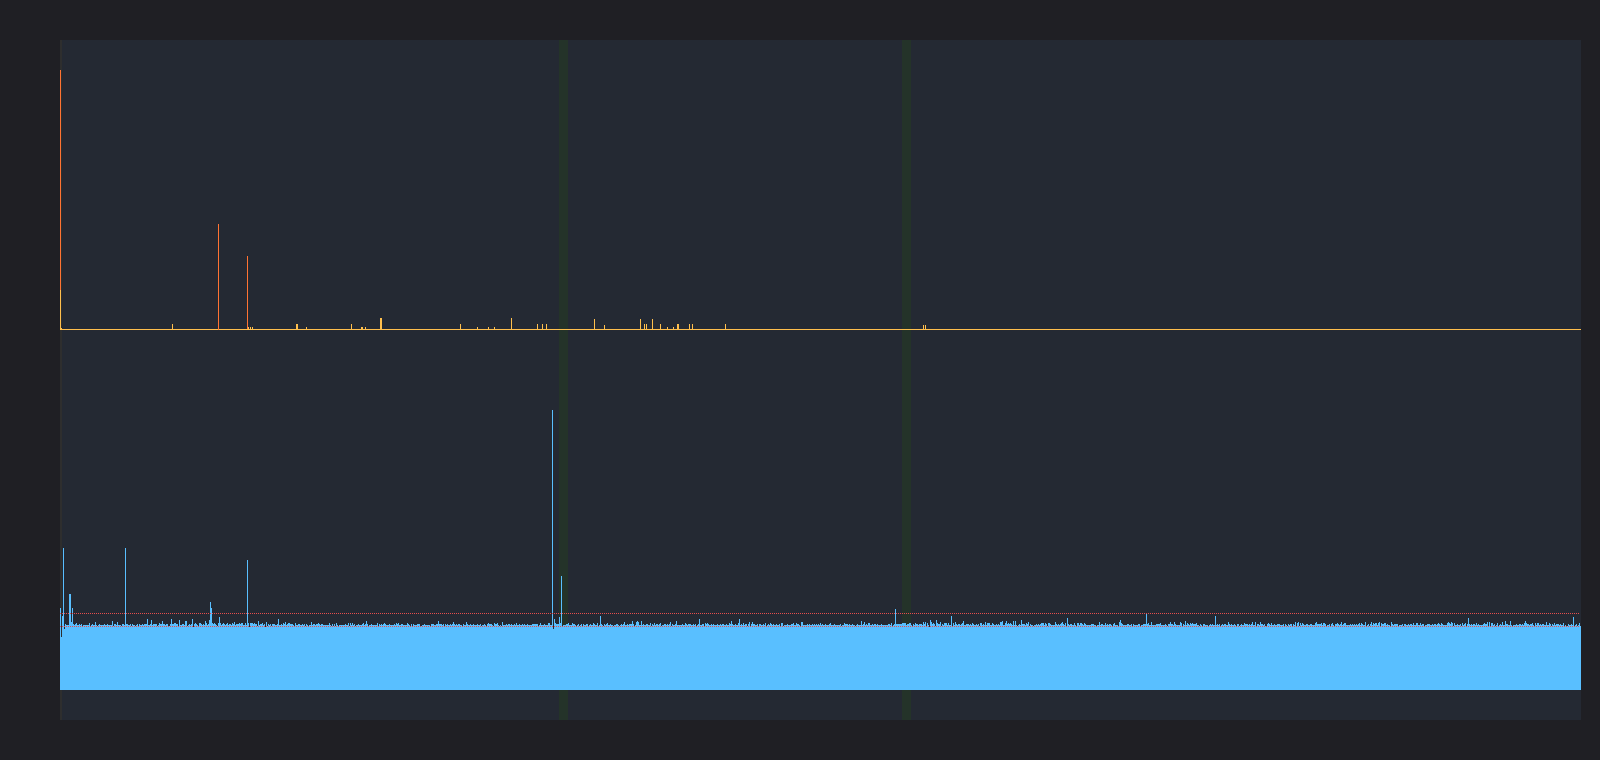
\includegraphics[width=\textwidth]{../captures-profiler/quest-apres-profiler-synthese.png}
\caption{Graphiques des mesures \texttt{ProfilerRecorder} (Quest avant / après).
Haut : mémoire allouée par frame (ko ; orange si $>$100~ko). Bas : temps CPU par frame
(ms ; lignes rouges = 13,9~ms pour 72~fps et 16,7~ms pour 60~fps ; échelle limitée à
60~ms). Fond : bleu = partie, vert = menu.}
\end{figure}

\begin{figure}[H]
\centering
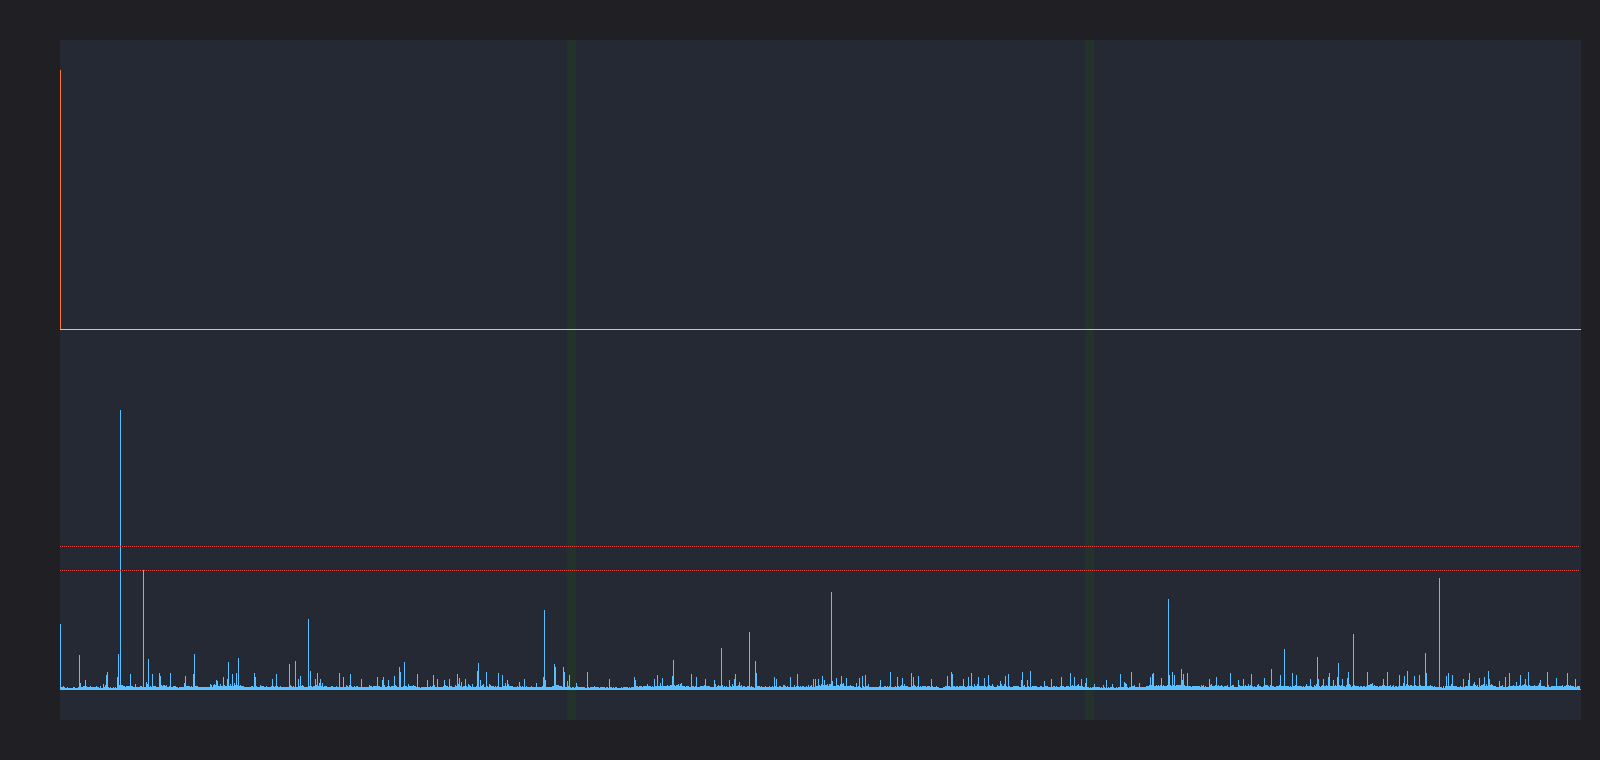
\includegraphics[width=\textwidth]{../captures-profiler/playmode-apres-profiler-synthese.png}
\caption{Bench « après » en Play Mode dans l'éditeur sur PC (sans casque). 3 parties
de 34 coupes, score 815 : identique au build Windows.}
\end{figure}

% =====================================================================
\section{Tests}\label{sec:tests}

\subsection{Vérifié sans casque}

\begin{itemize}
\item Compilation : 0 erreur à chaque étape. Audit projet inchangé : 1 script manquant
      préexistant dans une scène de test hors build, 1 shader non URP sur un
      \texttt{.dae} source hors build.
\item Builds Windows Development à chaque étape ; APK Quest Development avant/après
      (IL2CPP + ARM64 + OpenXR, 0 erreur, 75,4 / 76,4~Mo).
\item Bench PC, 3 parties : mêmes 34 coupes, 3 touches, 1 explosion par partie. Aucun
      état résiduel. Compteurs de pools cohérents : créations = stocks, pics $\le$ stocks.
\item Test d'échec Addressables : repli fonctionnel, même score (section 4).
\item Contenu Addressables : bundles PCVR seuls dans le build Windows, Quest seuls
      dans l'APK (vérifié dans \texttt{StreamingAssets/aa/}).
\end{itemize}

\subsection{Session casque du 25/11}

\begin{itemize}
\item APK « avant » installé, bench 3 parties $\times$ 3 runs. Les runs interrompus
      par la veille du casque sont écartés. Fichiers :
      \fichier{docs/part2/mesures-avant-quest/}.
\item APK « après » corrigé pendant la session (voir les limites), bench 3 parties.
      Fichiers : \fichier{docs/part2/mesures-apres-quest/}. Logs vérifiés :
      \texttt{[KatanaVariant] Variante 'Katana\_Quest' appliquée à 2 sabre(s)
      (132 sommets)}, \texttt{fallback=False handles=3}, \texttt{[GameFX] variante
      utilisée : Quest}.
\item Jeu libre Quest (utilisateur, casque porté) : 31 coupes réelles au katana
      (vitesses 1,1 à 2,6~m/s), 2 parties (Difficile puis Normal), touches de bombe
      1/3 et 2/3, retour menu. Les logs s'arrêtent là : le casque a été reposé.
\item Extras d'intent Android confirmés au casque (\texttt{-e bench 1} sur
      \texttt{UnityPlayerGameActivity}). Le fichier de secours \texttt{bench.flag}
      n'a pas été nécessaire.
\end{itemize}

Tests visuels : confirmé par l'utilisateur (déclaratif). L'utilisateur a
répondu « tout OK » pour les quatre points Quest : jus à la couleur du fruit à chaque
coupe ; explosion complète (shake + flash) à la 3e touche ; katana Quest ; plusieurs
parties sans fruit fantôme ni ralentissement. Il a aussi confirmé le test PCVR via
Link : variante PCVR des effets, katana détaillé. Les logs Quest ne montrent que
2 parties et 2 touches de bombe avant la veille du casque, et le test PCVR n'apparaît
pas dans les logs. La confirmation repose donc sur le déclaratif de l'utilisateur.
Les captures d'écran Quest étaient impossibles via adb (\texttt{screencap} bloqué
sur Quest 3, fichier 0 octet).

% =====================================================================
\section{Difficultés et limites}

\begin{itemize}
\item Extras Android : les extras \texttt{am start -e unity \ldots} n'arrivent pas
      dans \texttt{GetCommandLineArgs()}. Le bench lit les extras d'intent via
      \texttt{UnityPlayer.currentActivity}. Confirmé au casque. L'activité est
      \texttt{UnityPlayerGameActivity} (Unity 6), pas \texttt{UnityPlayerActivity}.
\item Défaut trouvé et corrigé en session casque : le groupe \texttt{FX\_Quest} était
      enregistré avec 2 entrées au lieu de 3. L'entrée Katana avait disparu après
      \texttt{CreateOrMoveEntry}, sans erreur dans les logs. Le catalogue Quest ne
      contenait donc pas le katana. Au casque : échec \texttt{ChainOperation failed},
      puis repli sur \texttt{Katana\_PCVR} (le mesh détaillé, sur Quest).
      \texttt{AddressablesSetup} vérifie maintenant chaque entrée après sauvegarde
      (re-création, et échec visible si elle ne tient pas). Contenu Quest et APK
      reconstruits, catalogue vérifié : \texttt{Katana\_Quest} appliqué au casque
      (132 sommets). L'APK défectueux est archivé.
\item Veille du Quest : le capteur de proximité endort l'app dès que le casque est
      posé. Un run interrompu donne des parties tronquées et des scores faux.
      \texttt{svc power stayon true} et le timeout Android n'y changent rien. Le casque
      doit être porté pendant le bench. Les runs interrompus sont écartés.
\item Scénario Quest $\neq$ PC : à 72~fps, les fruits montent moins haut entre deux
      frames et passent moins de temps au-dessus du seuil de coupe ($y \ge 0{,}3$).
      Les parties se terminent sur les 3 vies perdues : 13 à 37 coupes par partie
      selon les runs, contre 34 sur PC à $\sim$2500~fps. La comparaison avant/après
      Quest est normalisée par coupe et par minute. La comparaison Quest contre PC
      ne l'est pas.
\item Captures Profiler : la connexion Profiler$\rightarrow$Quest n'a pas pu être
      faite (éditeur Unity fermé pendant les runs Quest). \texttt{adb screencap}
      produit un fichier vide sur Quest 3 (restriction Meta). Les figures sont des
      graphiques tracés depuis les mesures \texttt{ProfilerRecorder}, plus un run
      Play Mode sur PC en repli. Ce ne sont pas des captures d'écran du Profiler.
\item État résiduel des bombes : l'« avant » laissait les bombes explosées figées
      dans la scène, et le bench les re-touchait gratuitement. La correction change
      le score de référence : 895 $\rightarrow$ 815.
\item Quad de flash de la bombe : parenté à la caméra, il survivait au retour au
      pool. Il est maintenant réutilisé entre explosions (un seul matériau par bombe)
      et détruit à la destruction finale.
\item Decimation du katana : faite par clustering dans l'éditeur, sans outil externe.
      Le maillage simplifié n'a pas de correspondance de sommets exacte avec
      l'original. C'est acceptable pour une arme vue en main. Le \texttt{MeshCollider}
      trigger du sabre est réassigné au mesh simplifié (la découpe utilise le plan de
      coupe, pas le mesh).
\item Limites du bench : sans casque, le CPU est dominé par le rendu
      \texttt{-nographics} et la simulation. Les gains du pooling sur le thread de
      rendu et la mémoire GPU ne se mesurent qu'au casque. Le scénario ne couvre pas
      les difficultés Hard/Extreme (stocks dimensionnés pour Normal, croissance
      possible).
\item Mesures Quest : avant $\times 3$ runs, après $\times 1$ run de référence (casque
      porté). La reproductibilité entre runs n'a pas pu être vérifiée côté après
      (veille du casque). Tests visuels confirmés par l'utilisateur (déclaratif),
      logs partiels (section~\ref{sec:tests}).
\end{itemize}

\end{document}